% Options for packages loaded elsewhere
% Options for packages loaded elsewhere
\PassOptionsToPackage{unicode}{hyperref}
\PassOptionsToPackage{hyphens}{url}
\PassOptionsToPackage{dvipsnames,svgnames,x11names}{xcolor}
%
\documentclass[
  12pt]{article}
\usepackage{xcolor}
\usepackage[margin=1in]{geometry}
\usepackage{amsmath,amssymb}
\setcounter{secnumdepth}{2}
\usepackage{iftex}
\ifPDFTeX
  \usepackage[T1]{fontenc}
  \usepackage[utf8]{inputenc}
  \usepackage{textcomp} % provide euro and other symbols
\else % if luatex or xetex
  \usepackage{unicode-math} % this also loads fontspec
  \defaultfontfeatures{Scale=MatchLowercase}
  \defaultfontfeatures[\rmfamily]{Ligatures=TeX,Scale=1}
\fi
\usepackage{lmodern}
\ifPDFTeX\else
  % xetex/luatex font selection
\fi
% Use upquote if available, for straight quotes in verbatim environments
\IfFileExists{upquote.sty}{\usepackage{upquote}}{}
\IfFileExists{microtype.sty}{% use microtype if available
  \usepackage[]{microtype}
  \UseMicrotypeSet[protrusion]{basicmath} % disable protrusion for tt fonts
}{}
\usepackage{setspace}
\makeatletter
\@ifundefined{KOMAClassName}{% if non-KOMA class
  \IfFileExists{parskip.sty}{%
    \usepackage{parskip}
  }{% else
    \setlength{\parindent}{0pt}
    \setlength{\parskip}{6pt plus 2pt minus 1pt}}
}{% if KOMA class
  \KOMAoptions{parskip=half}}
\makeatother
% Make \paragraph and \subparagraph free-standing
\makeatletter
\ifx\paragraph\undefined\else
  \let\oldparagraph\paragraph
  \renewcommand{\paragraph}{
    \@ifstar
      \xxxParagraphStar
      \xxxParagraphNoStar
  }
  \newcommand{\xxxParagraphStar}[1]{\oldparagraph*{#1}\mbox{}}
  \newcommand{\xxxParagraphNoStar}[1]{\oldparagraph{#1}\mbox{}}
\fi
\ifx\subparagraph\undefined\else
  \let\oldsubparagraph\subparagraph
  \renewcommand{\subparagraph}{
    \@ifstar
      \xxxSubParagraphStar
      \xxxSubParagraphNoStar
  }
  \newcommand{\xxxSubParagraphStar}[1]{\oldsubparagraph*{#1}\mbox{}}
  \newcommand{\xxxSubParagraphNoStar}[1]{\oldsubparagraph{#1}\mbox{}}
\fi
\makeatother


\usepackage{longtable,booktabs,array}
\usepackage{calc} % for calculating minipage widths
% Correct order of tables after \paragraph or \subparagraph
\usepackage{etoolbox}
\makeatletter
\patchcmd\longtable{\par}{\if@noskipsec\mbox{}\fi\par}{}{}
\makeatother
% Allow footnotes in longtable head/foot
\IfFileExists{footnotehyper.sty}{\usepackage{footnotehyper}}{\usepackage{footnote}}
\makesavenoteenv{longtable}
\usepackage{graphicx}
\makeatletter
\newsavebox\pandoc@box
\newcommand*\pandocbounded[1]{% scales image to fit in text height/width
  \sbox\pandoc@box{#1}%
  \Gscale@div\@tempa{\textheight}{\dimexpr\ht\pandoc@box+\dp\pandoc@box\relax}%
  \Gscale@div\@tempb{\linewidth}{\wd\pandoc@box}%
  \ifdim\@tempb\p@<\@tempa\p@\let\@tempa\@tempb\fi% select the smaller of both
  \ifdim\@tempa\p@<\p@\scalebox{\@tempa}{\usebox\pandoc@box}%
  \else\usebox{\pandoc@box}%
  \fi%
}
% Set default figure placement to htbp
\def\fps@figure{htbp}
\makeatother





\setlength{\emergencystretch}{3em} % prevent overfull lines

\providecommand{\tightlist}{%
  \setlength{\itemsep}{0pt}\setlength{\parskip}{0pt}}



 
\usepackage[]{natbib}
\bibliographystyle{ecca}


\usepackage{booktabs}
\usepackage{graphicx}
\usepackage{caption}
\usepackage{subcaption}
\usepackage{float}
\usepackage[section]{placeins}
\usepackage[dvipsnames]{xcolor}
% The following result macros are inlined from
% ../NHK-replications/meta_analysis_expanded/paper_macros.tex so that this
% submission source does not depend on generated TeX files.
\newcommand{\aiAnalyticN}{156}
\newcommand{\aiAttemptedRuns}{156}
\newcommand{\aiClaudeSonnetIqrLower}{$-0.005$}
\newcommand{\aiClaudeSonnetIqrUpper}{$0.132$}
\newcommand{\aiClaudeSonnetMean}{$0.069$}
\newcommand{\aiClaudeSonnetMedian}{$0.075$}
\newcommand{\aiClaudeSonnetN}{20}
\newcommand{\aiClaudeSonnetSd}{$0.089$}
\newcommand{\aiClusterStateShare}{$77.6$}
\newcommand{\aiDroppedRuns}{0}
\newcommand{\aiExcludedModelRuns}{40}
\newcommand{\aiFailedValidationRuns}{0}
\newcommand{\aiGptMiniIqrLower}{$0.015$}
\newcommand{\aiGptMiniIqrUpper}{$0.092$}
\newcommand{\aiGptMiniMean}{$0.064$}
\newcommand{\aiGptMiniMedian}{$0.036$}
\newcommand{\aiGptMiniN}{136}
\newcommand{\aiGptMiniSd}{$0.084$}
\newcommand{\aiIqrLower}{$0.014$}
\newcommand{\aiIqrUpper}{$0.099$}
\newcommand{\aiIqrWidth}{$0.084$}
\newcommand{\aiLinearModelShare}{$100.0$}
\newcommand{\aiMeanEffect}{$0.064$}
\newcommand{\aiMedianEffect}{$0.037$}
\newcommand{\aiMissingSpecRuns}{0}
\newcommand{\aiNoResultsRuns}{0}
\newcommand{\aiNoStateFeMean}{$0.056$}
\newcommand{\aiNoYearFeMean}{$0.051$}
\newcommand{\aiNonpositiveSeRuns}{0}
\newcommand{\aiOutlierRuns}{0}
\newcommand{\aiPerwtShare}{$87.8$}
\newcommand{\aiRecoverableSpecs}{156}
\newcommand{\aiSampleMax}{636,722}
\newcommand{\aiSampleMin}{1,764}
\newcommand{\aiSeMean}{$0.008$}
\newcommand{\aiSigFivePctFraction}{$0.897$}
\newcommand{\aiSigTenPctFraction}{$0.923$}
\newcommand{\aiStateFeMean}{$0.065$}
\newcommand{\aiStateFeShare}{$91.7$}
\newcommand{\aiWeightedMeanEffect}{$0.060$}
\newcommand{\aiYearFeMean}{$0.065$}
\newcommand{\aiYearFeShare}{$91.0$}
\newcommand{\benchmarkEffectN}{145}
\newcommand{\benchmarkIqrLower}{$0.014$}
\newcommand{\benchmarkIqrUpper}{$0.051$}
\newcommand{\benchmarkIqrWidth}{$0.037$}
\newcommand{\benchmarkMeanEffect}{$0.053$}
\newcommand{\benchmarkMedianEffect}{$0.030$}

% Inlined from LLM_replications_wordcount.tex.
\newcommand{\MainTextWordCount}{1,997}
\newcommand{\titleaffiliation}{Collegio Carlo Alberto}
\newcommand{\titlefirstdraft}{First draft: April 10, 2026}
\newcommand{\titledate}{This draft: \today}
\newcommand{\titlenote}{brett.mccully@carloalberto.org. I thank Yagan Hazard for helpful conversations. Any errors are my own.}
\makeatletter
\renewcommand{\maketitle}{
  \thispagestyle{empty}
  \begin{center}
  {\LARGE \@title\textsuperscript{*} \par}
  \vspace{1.5em}
  {\large \@author \par}
  \vspace{0.5em}
  {\normalsize \titleaffiliation \par}
  \vspace{0.75em}
  {\normalsize \titlefirstdraft \par}
  \vspace{0.25em}
  {\normalsize \titledate \par}
 % \vspace{0.75em}
 % {\footnotesize \textit{Word count (main text):} \MainTextWordCount \par}
  \end{center}
  \vspace{1.5em}
}
\makeatother
\makeatletter
\@ifpackageloaded{caption}{}{\usepackage{caption}}
\AtBeginDocument{%
\ifdefined\contentsname
  \renewcommand*\contentsname{Table of contents}
\else
  \newcommand\contentsname{Table of contents}
\fi
\ifdefined\listfigurename
  \renewcommand*\listfigurename{List of Figures}
\else
  \newcommand\listfigurename{List of Figures}
\fi
\ifdefined\listtablename
  \renewcommand*\listtablename{List of Tables}
\else
  \newcommand\listtablename{List of Tables}
\fi
\ifdefined\figurename
  \renewcommand*\figurename{Figure}
\else
  \newcommand\figurename{Figure}
\fi
\ifdefined\tablename
  \renewcommand*\tablename{Table}
\else
  \newcommand\tablename{Table}
\fi
}
\@ifpackageloaded{float}{}{\usepackage{float}}
\floatstyle{ruled}
\@ifundefined{c@chapter}{\newfloat{codelisting}{h}{lop}}{\newfloat{codelisting}{h}{lop}[chapter]}
\floatname{codelisting}{Listing}
\newcommand*\listoflistings{\listof{codelisting}{List of Listings}}
\makeatother
\makeatletter
\makeatother
\makeatletter
\@ifpackageloaded{caption}{}{\usepackage{caption}}
\@ifpackageloaded{subcaption}{}{\usepackage{subcaption}}
\makeatother
\usepackage{bookmark}
\IfFileExists{xurl.sty}{\usepackage{xurl}}{} % add URL line breaks if available
\urlstyle{same}
\hypersetup{
  pdftitle={Research Choices of Agentic Artificial Intelligence},
  pdfauthor={Brett A. McCully},
  colorlinks=true,
  linkcolor={blue},
  filecolor={Maroon},
  citecolor={Blue},
  urlcolor={Blue},
  pdfcreator={LaTeX via pandoc}}


\title{Research Choices of Agentic Artificial Intelligence}
\author{Brett A. McCully}
\date{2026-07-31}
\begin{document}
\maketitle
\begin{abstract}
Researchers increasingly rely on agentic artificial intelligence to
assist with research. I examine the sampling and specification choices
AI agents make and compare them to those of human experts. Fixing the
research question and raw data across 156 agent runs, AIs tend to
cluster on certain options. Compared to 145 human expert analyses of the
same question and data, estimation outcomes are broadly similar. AI
achieves this, however, via systematically different choices. Agentic AI
thus remains an imperfect substitute for human researchers for the
models tested.
\end{abstract}


\setstretch{1.5}
\begin{quotation}
\footnotesize
\noindent \textbf{Keywords:} AI agents, LLMs, multi-analyst studies

\medskip
\noindent \textbf{JEL Codes:} C6, C18, C88
\end{quotation}

\vfill
\noindent\rule{0.33\textwidth}{0.4pt}
\par
\noindent {\footnotesize \textsuperscript{*}\titlenote\par}

\newpage

\section{Introduction}\label{sec-intro}

Recent advances in artificial intelligence are transforming the way
research is done. Economists increasingly use agentic AI, such as Claude
Code and Codex, to clean and analyze
data.\footnote{A straw poll during the NBER Summer Institute for Household Finance revealed approximately 60\% of economists are `all-in' on agentic AI, see \url{https://x.com/S_Stantcheva/status/2080706102044291124}.}
Some are testing the extent to which agentic AI can automate the entire
research pipeline from idea to paper
\citep{projectape2026, willner2026verifying}. The rise of AI agent use
makes verification of AI output the bottleneck: ensuring AI research
choices are appropriate and match with the preferences of the human
expert \citep{korinek2025ai}. Systematic evidence on the research
choices of AI, however, is lacking.

In this paper, I examine AI agents' sampling and specification decisions
and the corresponding estimation results. I then assess how well these
choices compare to those of human experts. To this end, I direct 156 AI
agents to answer the same question studied by many human analysts in
\citet{huntingtonklein2025sources}: how eligibility for the Deferred
Action for Childhood Arrivals program affects the probability of
full-time employment for eligible workers. Each agent receives the same
research prompt and raw dataset but independently generates a complete
empirical specification---sample restrictions, estimating equation, and
standard errors. The inherent stochasticity of the large language models
that power modern AI agents ensures there is variation in research
choices, though to what degree is not well understood.

Sampling and specification choices sharply differ between AI agents and
human experts. At many forking paths, such as which regression method to
use or whether to use sampling weights, AI agents overwhelming make the
same decision, despite AI agents' underlying stochasticity. By contrast,
there is substantially more variation in the decisions human experts
make at the same forking paths. Despite these differences, the AI
agents' distributions of estimation outcomes broadly resemble those of
the human experts. Overall, my findings underline why researchers should
review the data cleaning and analysis decisions of AI, as there is a
strong likelihood that some of these choices may not line up with one's
own preference.

A growing body of evidence shows that researchers answering the same
question and using the same raw data make different decisions that can
produce meaningfully different estimates
\citep{silberzahn2018many, huntington2021influence, breznau2022observing}.
The present study is one of several this year to examine variation in
agentic AI estimates: \citet{gao2026nonstandard},
\citet{grundl2026comparison}, and \citet{huang2026aierrors}. Among these
papers, only \citet{grundl2026comparison} looks at the study by
\citet{huntingtonklein2025sources}, and he does not focus on agent
choices as I do.

\section{Method}\label{sec-method}

\subsection{AI agents as empirical
researchers}\label{ai-agents-as-empirical-researchers}

Large language models give non-deterministic responses: the same prompt
can generate a range of responses. Submitting the same prompt to
estimate a given empirical parameter many times therefore yields a
distribution of AI choices.

AI agents may produce reasonable research choices because their
underlying models are trained on huge corpora of digital data
\citep{openai2025gpt5systemcard, anthropic2026systemcard}, almost surely
including much economics research and associated code. The language in
the prompt given to the AI agent (e.g., ``causal'' and a focus on labor
market outcomes) should nudge output toward the conventions of applied
economists, rather than, say, data science. AI outputs may therefore be
interpreted as draws from a noisy representation of standard practices
in economics. Alternatively, AI agents may make choices far outside
disciplinary norms, or less internally coherent ones. Given model
complexity, stochasticity, and closed-source nature, how closely AI
agents hew to human patterns is an empirical question.

\subsection{Application}\label{application}

I task AI agents with the same question answered by many human analysts
in \citet{huntingtonklein2025sources}. The authors retained 146 teams of
economists and asked each to independently answer the same causal
question using the same instructions and raw data: how did eligibility
for the Deferred Action for Childhood Arrivals immigration policy affect
the probability of full-time employment among eligible immigrants?
Participants were given a data codebook and the research question but
otherwise initially exercised broad discretion over sample construction,
variable definitions, and specification choices (called Task 1 in the
study).

The computing pipeline works as follows. An AI agent is provided with
the raw materials to answer the research question: an IPUMS extract and
codebook with a broad set of variables, a supplementary state policy
dataset and codebook, and instructions adapted from
\citet{huntingtonklein2025sources}.\footnote{Replication code and the AI agent results can be found at \url{https://github.com/brettmcc/LLM-bootstrapping/}.}
The agent then writes a concise, structured file outlining their model
specification, outcome definition, sample selection, and treatment
definition. They proceed to write and execute a Python script to
implement the estimation, working through any coding errors along the
way, and reporting the resulting coefficient estimate, standard error,
and sample size. Sampling and specification choices are then
programmatically scraped from agents' reports and cross-referenced
against the actual code they produced to ensure accuracy.

Access to IPUMS differed between the two groups. Humans were instructed
to navigate to the IPUMS website and select the variables they thought
relevant. In contrast, AI agents received a fixed IPUMS extract
containing all variables used by any of the human researchers, obtained
by scanning the repository of human submissions to
\citet{huntingtonklein2025sources} hosted by Open Science Framework.
This restricts AI agents from choosing any variable whatsoever, but
still leaves substantial latitude in variable
selection.\footnote{An alternative would have been to give each AI agent access to the IPUMS API via my personal API key. I opted against this both to avoid hundreds of large ACS files on my machine and to not overburden the IPUMS API.}

I used two then-frontier medium-sized AI models---GPT-5.4 mini (OpenAI)
and Claude Sonnet 4.6
(Anthropic)\footnote{I exclude \aiExcludedModelRuns{} exploratory runs with Claude's smaller and less advanced Haiku 4.5 model, which yielded several degenerate results, such as a standard error of 0. Researchers applying this approach should therefore take heed that weaker models may not be suitable for this type of task.}---accessed
through the GitHub Copilot CLI. I primarily rely on GPT-5.4 mini, as it
is cheaper to run than Claude Sonnet 4.6. When using a subscription such
as Codex or Claude Code, the marginal cost of each run is modest, making
the exercise more affordable for individual researchers.

\section{Results}\label{sec-results}

I explore \aiAnalyticN{} AI agent analyses and compare them to 145 human
analyses from \citet{huntingtonklein2025sources}. Both humans and agents
had substantial freedom to over sample selection, variable definitions,
and specification.

\subsection{Choices of AI and Humans}\label{choices-of-ai-and-humans}

Table \ref{tab:methods} displays the prevalence of model specification
choices between AI and human runs.

% Inlined from paper_table2_methods.tex and its nested table4_method_shares.tex.
\begin{table}[!htbp]
\centering
\caption{Estimation choices by researcher type}
\label{tab:methods}
\small
\resizebox{\textwidth}{!}{%
\begin{tabular}{@{}l l r r r r@{}}
\toprule
 &  & \multicolumn{2}{c}{AI} & \multicolumn{2}{c}{Humans} \\
\cmidrule(lr){3-4}\cmidrule(lr){5-6}
Category & Choice & N & Share (\%) & N & Share (\%) \\
\midrule
Method & Linear Regression & 156 & 100.0 & 122 & 84.1 \\
 & Logit/Probit & 0 & 0.0 & 19 & 13.1 \\
 & Matching & 0 & 0.0 & 2 & 1.4 \\
 & New DID Estimator & 0 & 0.0 & 1 & 0.7 \\
 & Other & 0 & 0.0 & 1 & 0.7 \\
S.E. Adjustment & Cluster (State) & 127 & 81.4 & 31 & 21.2 \\
 & Cluster (State \& Year) & 1 & 0.6 & 22 & 15.1 \\
 & Cluster (ID/Strata/Other) & 0 & 0.0 & 20 & 13.7 \\
 & Het-Robust & 26 & 16.7 & 24 & 16.4 \\
 & Other/Bootstrap & 0 & 0.0 & 7 & 4.8 \\
 & None & 2 & 1.3 & 42 & 28.8 \\
Weights & No Sample Weights & 7 & 4.5 & 101 & 69.2 \\
 & Sample Weights & 149 & 95.5 & 45 & 30.8 \\
\bottomrule
\end{tabular} }
\caption*{\footnotesize \textbf{Notes:} Estimation choices are inferred from each generated model specification and execution metadata. Human results use Task 1 submissions from \citet{huntingtonklein2025sources}.}
\end{table}
\FloatBarrier

I find that AI agents exhibit little to no variation in their
specification choices, sharply contrasting with humans. AI agents
exclusively chose linear models, in contrast to 13\% of human runs using
nonlinear models. AI agents also overwhelmingly converged on clustering
standard errors at the state level, with 81\% of agents choosing to do
so compared to 21\% of human runs. The share of runs featuring
heteroskedasticity robust standard errors was quite similar between AI
and humans.

One concern is that differences the programming language used may
contribute to differences in research choices. Most humans used Stata or
R, while I required the AI to use Python. Default standard error
computation differs across languages, and AI may go with default
settings. Instead, 98.7\% of AI agents actively chose a standard error
method rather than relying on the
default.\footnote{This contrasts with the excluded AI runs executed by the less intelligent Claude Haiku 4.5, which heavily relied on the default standard error method.}
What I cannot rule out is that observed empirical practices may have
differed by language in the AI model's training data, and these
differences may affect the observed choices.

AI agents almost exclusively used sample weights, while a majority of
human researchers did not. Using weights is in line with IPUMS
instructions, a fact highlighted by \citet{huntingtonklein2025sources}.

Choice of control variables differed substantially between humans and
AI, as shown in Table \ref{tab:controls}. AI agents included an age
control more frequently than humans did, and AI almost never controlled
for education while humans did in nearly half of specifications. 92\% of
AI agents included year fixed effects, compared to just 27\% of human
runs. Similarly, 92\% of AIs included state fixed effects compared to
36\% of human runs. Estimating a fully-saturated
difference-in-differences specification diminishes the downsides of
linear probability models, the choice of every AI agent, as noted by
\citet{huntingtonklein2025sources}. Overall, AI agents agreed on the set
of controls much more often than human researchers. Just 25\% of AI
agent runs used a set of controls unique among all other AIs, compared
to 60\% of humans.

\begin{table}[!htbp]
\centering
\caption{Control variable choices by researcher type}
\label{tab:controls}
\small
\resizebox{\textwidth}{!}{%
\begin{tabular}{@{}l l r r r r@{}}
\toprule
 &  & \multicolumn{2}{c}{AI} & \multicolumn{2}{c}{Humans} \\
\cmidrule(lr){3-4}\cmidrule(lr){5-6}
Category & Control & N & Share (\%) & N & Share (\%) \\
\midrule
AGE & Linear Age & 82 & 52.6 & 61 & 41.8 \\
AGE & Age FE & 19 & 12.2 & 13 & 8.9 \\
AGE & Age Quadratic & 69 & 44.2 & 11 & 7.5 \\
EDUC & Linear Education & 3 & 1.9 & 46 & 31.5 \\
EDUC & Education FE & 1 & 0.6 & 8 & 5.5 \\
EDUC & Education Transform & 0 & 0.0 & 16 & 11.0 \\
STATE/YEAR & Linear Year & 16 & 10.3 & 33 & 22.6 \\
STATE/YEAR & Year FE & 143 & 91.7 & 40 & 27.4 \\
STATE/YEAR & State FE & 144 & 92.3 & 52 & 35.6 \\
STATE/YEAR & State FE x Year FE & 132 & 84.6 & 19 & 13.0 \\
STATE/YEAR & State FE x Linear Year & 15 & 9.6 & 5 & 3.4 \\
\bottomrule
\end{tabular} }
\caption*{\footnotesize \textbf{Notes:} The table presents the number and share of AI and human estimation specifications that included various controls. Human results use Task 1 submissions from \citet{huntingtonklein2025sources}.}
\end{table}
\FloatBarrier

Next, Table \ref{tab:sample-restrictions} compares sample and treated
group filters. Rows underneath each variable heading are roughly ordered
by the `correctness' for defining the treated group, as in
\citet{huntingtonklein2025sources}. This is based on DACA's eligibility
criteria, which are listed in the AI's prompt. The prompt does not
specify, however, how to construct the control
group.\footnote{In prompting the AI, I did not mention restricting the sample based on education or veteran status, consistent with the prompt given to the human researchers in Task 1 by \citet{huntingtonklein2025sources}.}

\begin{table}[H]
\centering
\caption{Sample and treated-group restriction choices by researcher type}
\label{tab:sample-restrictions}
\tiny
\setlength{\tabcolsep}{1.4pt}
\renewcommand{\arraystretch}{0.55}
\resizebox{\textwidth}{!}{%
\begin{tabular}{lrcrcrcrc}
\toprule
Variable & \multicolumn{4}{c}{AI} & \multicolumn{4}{c}{Humans} \\
\cmidrule(lr){2-5}\cmidrule(lr){6-9}
& \multicolumn{2}{c}{All} & \multicolumn{2}{c}{Treated} & \multicolumn{2}{c}{All} & \multicolumn{2}{c}{Treated} \\
\cmidrule(lr){2-3}\cmidrule(lr){4-5}\cmidrule(lr){6-7}\cmidrule(lr){8-9}
& N & Share (\%) & N & Share (\%) & N & Share (\%) & N & Share (\%) \\
\midrule
Hispanic & 156 & & 156 & & 144 & & 144 & \\
... Hispanic-Mexican & 154 & 98.7 & 154 & 98.7 & 105 & 72.9 & 109 & 75.7 \\
... Hispanic-Any & 2 & 1.3 & 2 & 1.3 & 17 & 11.8 & 17 & 11.8 \\
... Hispanic-Mex or Mex-Born & 0 & 0.0 & 0 & 0.0 & 1 & 0.7 & 2 & 1.4 \\
... None & 0 & 0.0 & 0 & 0.0 & 21 & 14.6 & 16 & 11.1 \\
Birthplace & 156 & & 156 & & 145 & & 145 & \\
... Mexican-Born & 154 & 98.7 & 154 & 98.7 & 103 & 71.0 & 112 & 77.2 \\
... Hispanic-Mex or Mex-Born & 0 & 0.0 & 0 & 0.0 & 2 & 1.4 & 2 & 1.4 \\
... Non-US Born & 0 & 0.0 & 0 & 0.0 & 4 & 2.8 & 4 & 2.8 \\
... Central America-Born & 0 & 0.0 & 0 & 0.0 & 1 & 0.7 & 1 & 0.7 \\
... None & 2 & 1.3 & 2 & 1.3 & 35 & 24.1 & 26 & 17.9 \\
Citizenship & 156 & & 156 & & 145 & & 145 & \\
... Non-Citizen & 153 & 98.1 & 153 & 98.1 & 83 & 57.2 & 117 & 80.7 \\
... Foreign-Born & 2 & 1.3 & 2 & 1.3 & 2 & 1.4 & 2 & 1.4 \\
... Non-Cit or Natlzd post-2012 & 0 & 0.0 & 0 & 0.0 & 4 & 2.8 & 7 & 4.8 \\
... Other & 1 & 0.6 & 1 & 0.6 & 11 & 7.6 & 11 & 7.6 \\
... None & 0 & 0.0 & 0 & 0.0 & 45 & 31.0 & 8 & 5.5 \\
Age at Migration & 156 & & 156 & & 145 & & 145 & \\
... $<$ 16 & 56 & 35.9 & 112 & 71.8 & 21 & 14.5 & 105 & 72.4 \\
... $\leq$ 16 & 0 & 0.0 & 0 & 0.0 & 10 & 6.9 & 25 & 17.2 \\
... Other & 36 & 23.1 & 12 & 7.7 & 24 & 16.6 & 11 & 7.6 \\
... None & 64 & 41.0 & 32 & 20.5 & 90 & 62.1 & 4 & 2.8 \\
Age in June 2012 & 156 & & 156 & & 145 & & 145 & \\
... Year-Quarter Age & 6 & 3.8 & 11 & 7.1 & 40 & 27.6 & 117 & 80.7 \\
... Year-Only Age & 148 & 94.9 & 143 & 91.7 & 18 & 12.4 & 21 & 14.5 \\
... Other & 0 & 0.0 & 0 & 0.0 & 2 & 1.4 & 0 & 0.0 \\
... None & 2 & 1.3 & 2 & 1.3 & 85 & 58.6 & 7 & 4.8 \\
Year of Immigration & 156 & & 156 & & 145 & & 145 & \\
... $<$ 2007 & 0 & 0.0 & 0 & 0.0 & 15 & 10.3 & 43 & 29.7 \\
... $\leq$ 2007 & 78 & 50.0 & 133 & 85.3 & 13 & 9.0 & 52 & 35.9 \\
... $<$ 2012 & 0 & 0.0 & 0 & 0.0 & 3 & 2.1 & 1 & 0.7 \\
... $\leq$ 2012 & 0 & 0.0 & 0 & 0.0 & 2 & 1.4 & 4 & 2.8 \\
... Any Year & 44 & 28.2 & 9 & 5.8 & 7 & 4.8 & 4 & 2.8 \\
... Other & 26 & 16.7 & 9 & 5.8 & 5 & 3.4 & 3 & 2.1 \\
... None & 8 & 5.1 & 5 & 3.2 & 100 & 69.0 & 38 & 26.2 \\
Years Continuous in USA & 156 & & 156 & & 145 & & 145 & \\
... Used YRSUSA & 1 & 0.6 & 4 & 2.6 & 23 & 15.9 & 55 & 37.9 \\
... No YRSUSA & 155 & 99.4 & 152 & 97.4 & 122 & 84.1 & 90 & 62.1 \\
\bottomrule
\end{tabular} }
\caption*{\footnotesize \textbf{Notes:} The table compares AI-agent restriction choices with the published Task 1 counts from Table 6 of \citet{huntingtonklein2025sources}. Treated-group restrictions inherit those used to restrict the whole sample.}
\end{table}
\FloatBarrier

Once again AI agents overwhelmingly converged on several sample and
treated-group construction choices. Virtually all AI agents restricted
the sample to ethnically Hispanic-Mexicans born in Mexico who are not US
citizens.\footnote{I suspect this results from the AI becoming highly focused on the first clause of the AI prompt (copied verbatim from the human task), ``\textbf{Among ethnically Hispanic-Mexican Mexican-born people living in the United States}, what was the causal impact of eligibility for the Deferred Action for Childhood Arrivals (DACA) program (treatment) on the probability that the eligible person is employed full-time (outcome),'' emphasis mine.}

Moreover, AI consistently diverged from humans when coding treatment.
First, AI was much less likely to condition treatment on age derived
from both birth year and birth quarter (7\% vs.~humans' 81\%), instead
preferring age measured only in years. This lack of precision matters
because the DACA eligibility age cutoff is June 15, 2012, as conveyed in
the AI's prompt. Second, AI frequently includes immigrants arriving in
2007 as part of the treated group. DACA applied to those who lived
continuously in the US since June 15, 2007. AI never conditions
treatment on arrival prior to 2007 (0\% compared to humans' 30\%),
rather defining it conditional on arrival up to and including 2007 (85\%
of the time vs.~humans' 36\%). Relatedly, AI rarely used years of
continuous US residence in defining treatment (3\% vs.~humans' 38\%).
Hence AI is less conservative on average than humans in assigning DACA
eligibility, including more ineligible individuals in the treated group.

\subsection{Distribution of estimates}\label{distribution-of-estimates}

Despite sharp differences in sampling and specification choices, how do
the resulting estimation outcomes compare? Figure
\ref{fig:comparison-boxplots} depicts box-and-whisker plots for both
human and AI analyses for weighted and unweighted effects, standard
errors, and sample size. Exact values are reported in Table
\ref{tab:appendix-summary-nhk}.

\begin{center}
\begin{minipage}{\textwidth}
\centering
\captionof{figure}{Human and AI estimation outcomes}
\label{fig:comparison-boxplots}
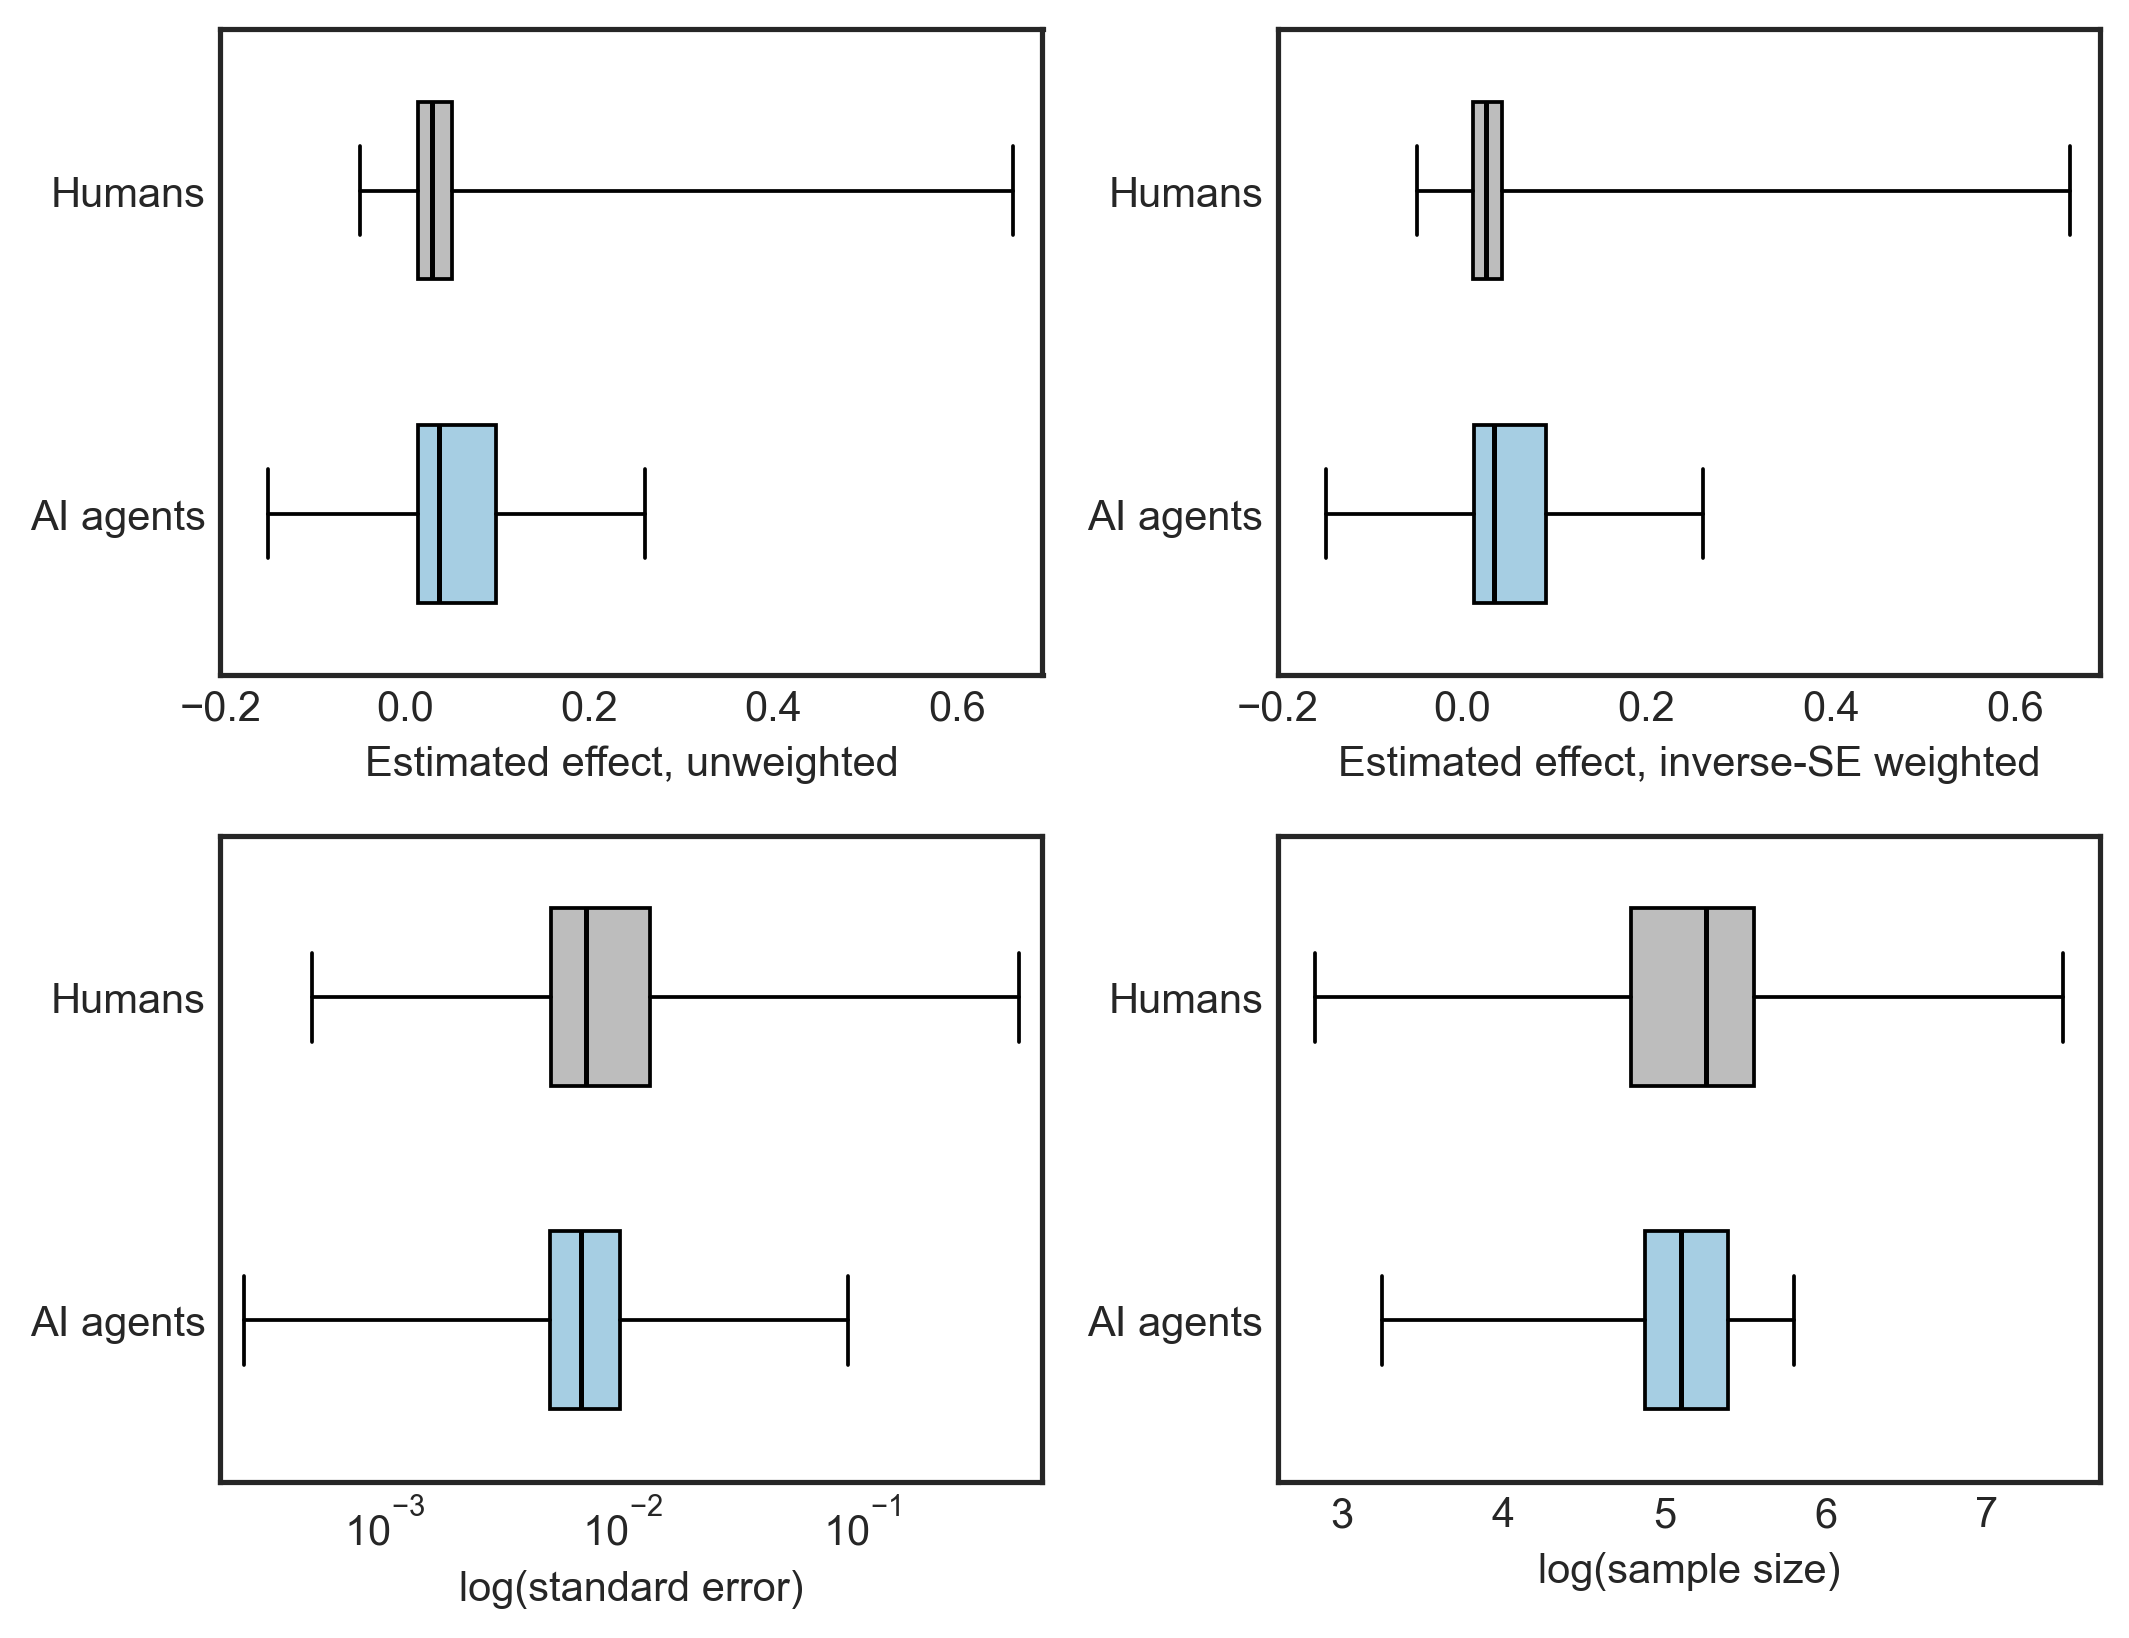
\includegraphics[width=0.82\textwidth]{../NHK-replications/meta_analysis_expanded/figure4_comparison_boxplots.png}
\captionof*{figure}{\scriptsize \textbf{Notes:} Panels compare unweighted point-estimate distributions (top left), point-estimate distributions weighted by inverse standard error (top right), standard errors (bottom left), and $\log$ sample sizes (bottom right) for both the human researcher sample of Task 1 from \citet{huntingtonklein2025sources} and the AI agent sample from this paper. In line with \citet{huntingtonklein2025sources}, inverse standard error weights are capped at the 95th percentile. Boxes show the interquartile range, center lines show medians, and whiskers show minimum and maximum values.}
\end{minipage}
\end{center}

Across all four outcomes, medians are fairly similar between human and
AI researchers. Moreover, AI agents exhibit substantial dispersion in
their estimation outcomes, underlining the stochasticity of AI outputs.

\begin{table}[!htbp]
\centering
\caption{Summary statistics on estimation outcomes}
\label{tab:appendix-summary-nhk}
\small
\resizebox{\textwidth}{!}{%
\begin{tabular}{@{}l r r r r r r r r@{}}
\toprule
 & N & Mean & SD & Min & Pctl. 25 & Median & Pctl. 75 & Max \\
\midrule
\multicolumn{9}{@{}l}{\textit{Panel A: AI-agent estimates}} \\
Effect Size (unweighted) & 156 & 0.064 & 0.084 & -0.148 & 0.014 & 0.037 & 0.099 & 0.261 \\
Effect Size (weighted by inverse SE) & 156 & 0.060 & 0.080 & -0.148 & 0.013 & 0.035 & 0.091 & 0.261 \\
Standard Error & 156 & 0.008 & 0.007 & 0.000 & 0.005 & 0.007 & 0.010 & 0.088 \\
Sample Size & 156 & 165,965 & 123,732 & 1,764 & 75,319 & 125,655 & 248,270 & 636,722 \\
Treated-Group Size & 155 & 65,518 & 28,865 & 7,717 & 36,477 & 74,231 & 81,508 & 169,320 \\
\addlinespace
\multicolumn{9}{@{}l}{\textit{Panel B: Human estimates}} \\
Effect Size (unweighted) & 145 & 0.053 & 0.095 & -0.049 & 0.014 & 0.030 & 0.051 & 0.660 \\
Effect Size (weighted by inverse SE) & 138 & 0.044 & 0.092 & -0.049 & 0.012 & 0.026 & 0.043 & 0.660 \\
Standard Error & 139 & 0.019 & 0.055 & 0.000 & 0.005 & 0.007 & 0.013 & 0.460 \\
Sample Size & 145 & 828,318 & 3,056,037 & 681 & 61,600 & 179,960 & 356,787 & 29,536,580 \\
Treated-Group Size & 141 & 96,395 & 648,493 & 270 & 17,950 & 34,435 & 52,581 & 7,727,201 \\
\bottomrule
\end{tabular} }
\caption*{\footnotesize \textbf{Notes:} Panel A reports outcomes from the AI agent sample. Panel B restates the published Task 1 panel of Table 3 of \citet{huntingtonklein2025sources}. Treated-group sample size not available for all AI agent runs since its collection was added after the initial runs.}
\end{table}

For the unweighted effect size plotted in the top left, AI runs yield a
mean of 0.064 and a median of \aiMedianEffect{} and humans a mean of
0.053 and median of \benchmarkMedianEffect{}. The 25th percentile
estimates are identical at 0.014, while the 75th percentile effect is
substantially larger for AI agents at 0.099 relative to humans' 0.051.
Results are quite similar for the inverse-standard error weighted
coefficients plotted in the top right.

Human point estimates exhibit a 13\% higher standard deviation in effect
size, driven by a much longer positive tail. The maximum human estimate
is 2.5 times the maximum AI estimate, while the minimum AI estimate is 3
times more negative than the minimum human estimate. Still, 92\% of AI
point estimates are within the min-max range of humans, and 30\% are
within humans' interquartile range.

For standard errors, plotted in the bottom left, the minimum, 25th
percentile, and median are identical across humans and AI, while human
estimates exhibit higher standard errors at the 75th percentile and
maximum. Correspondingly, AI agents obtain coefficients statistically
significantly different from 0 about 90\% of the time, compared to 78\%
of the time among humans.

The range of sample sizes chosen by human researchers---between 681 and
over 29 million observations---is several orders of magnitude larger
than what the AI agents chose. Still, the interquartile range is
comparable: 75 to 248 thousand for the AI, and 61 to 357 thousand for
the humans.

\section{Conclusion}\label{sec-conclusion}

This paper assesses the choices of agentic artificial intelligence and
how they compare to human experts'. I do so leveraging the multi-analyst
study of \citet{huntingtonklein2025sources}.

While AI agent estimation outcome distributions resemble those of
humans, the way in which each group arrives at those estimates differ
markedly. AI agents converged much more on particular specification and
sampling choices relative to human researchers. This finding is
consistent with concurrent work by \citet{huang2026aierrors}, who find
in a different setting that AI tends to cluster on certain sampling and
specification choices. Hence, I conclude that AI is thus far an
imperfect substitute for human experts.

Two limitations are worth emphasizing. First, the
\citet{huntingtonklein2025sources} materials were public before my runs,
so model training data may have included the original study or analyst
submissions. Still, the convergence of many AI choices in contrast to
the human analysts suggests the AI was not merely copying human work.
Second, results may depend on agent model and harness. Future work
should examine whether more advanced models, such as (at the time of
writing) GPT-5.6 and Claude Fable 5 can better match or even outperform
human experts.


% Bibliography inlined from the ecca.bst-formatted BibTeX output. This makes
% the submission independent of bibliography.bib and of a BibTeX build step.
\begin{thebibliography}{12}
\providecommand{\natexlab}[1]{#1}

\bibitem[{{Anthropic}(2026)}]{anthropic2026systemcard}
\textsc{{Anthropic}} (2026). System card: Claude sonnet 4.6.

\bibitem[{Breznau \textit{et~al.}(2022)Breznau, Rinke, Wuttke
  \textit{et~al.}}]{breznau2022observing}
\textsc{Breznau, N.}, \textsc{Rinke, M.~E.}, \textsc{Wuttke, A.}
  \textit{et~al.} (2022). Observing many researchers using the same data and
  hypothesis reveals a hidden universe of uncertainty. \textit{Proceedings of
  the National Academy of Sciences}, \textbf{119}~(44), e2203150119.

\bibitem[{Gao and Xiao(2026)}]{gao2026nonstandard}
\textsc{Gao, R.} and \textsc{Xiao, S.~C.} (2026). Nonstandard errors in {AI}
  agents. SSRN working paper, date written: March 16, 2026.

\bibitem[{Grundl(2026)}]{grundl2026comparison}
\textsc{Grundl, S.} (2026). A comparison of agentic {AI} systems and human
  economists. SSRN working paper, date written: April 9, 2026.

\bibitem[{Huang \textit{et~al.}(2026)Huang, Menkveld and
  Yu}]{huang2026aierrors}
\textsc{Huang, W.}, \textsc{Menkveld, A.~J.} and \textsc{Yu, S.} (2026). {AI}
  ``errors''. SSRN working paper, date written: March 13, 2026.

\bibitem[{Huntington-Klein \textit{et~al.}(2021)Huntington-Klein, Arenas, Beam,
  Bertoni, Bloem, Burli, Chen, Grieco, Ekpe, Pugatch
  \textit{et~al.}}]{huntington2021influence}
\textsc{Huntington-Klein, N.}, \textsc{Arenas, A.}, \textsc{Beam, E.},
  \textsc{Bertoni, M.}, \textsc{Bloem, J.~R.}, \textsc{Burli, P.},
  \textsc{Chen, N.}, \textsc{Grieco, P.}, \textsc{Ekpe, G.}, \textsc{Pugatch,
  T.} \textit{et~al.} (2021). The influence of hidden researcher decisions in
  applied microeconomics. \textit{Economic Inquiry}, \textbf{59}~(3), 944--960.

\bibitem[{Huntington-Klein \textit{et~al.}(2025)Huntington-Klein, Portner,
  McCarthy and {The Many Economists Collaborative on Researcher
  Variation}}]{huntingtonklein2025sources}
\textsc{---}, \textsc{Portner, C.~C.}, \textsc{McCarthy, I.} and \textsc{{The
  Many Economists Collaborative on Researcher Variation}} (2025). \textit{The
  Sources of Researcher Variation in Economics}. {I4R} Discussion Paper 209,
  Institute for Replication ({I4R}).

\bibitem[{Korinek(2025)}]{korinek2025ai}
\textsc{Korinek, A.} (2025). \textit{AI agents for economic research}. Tech.
  rep., National Bureau of Economic Research.

\bibitem[{{OpenAI}(2025)}]{openai2025gpt5systemcard}
\textsc{{OpenAI}} (2025). {GPT-5} system card.

\bibitem[{{Project APE}(2026)}]{projectape2026}
\textsc{{Project APE}} (2026). Project {APE}: Autonomous policy evaluation.
  Social Catalyst Lab, University of Zurich, accessed July 29, 2026.

\bibitem[{Silberzahn \textit{et~al.}(2018)Silberzahn, Uhlmann, Martin
  \textit{et~al.}}]{silberzahn2018many}
\textsc{Silberzahn, R.}, \textsc{Uhlmann, E.~L.}, \textsc{Martin, D.~P.}
  \textit{et~al.} (2018). Many analysts, one data set: Making transparent how
  variations in analytic choices affect results. \textit{Advances in Methods
  and Practices in Psychological Science}, \textbf{1}~(3), 337--356.

\bibitem[{Willner and Yanagizawa-Drott(2026)}]{willner2026verifying}
\textsc{Willner, O.} and \textsc{Yanagizawa-Drott, D.} (2026). Verifying the
  verifiers: Towards autonomous policy evaluation, working paper, July 20,
  2026.

\end{thebibliography}



\end{document}
